\frame{\frametitle{Low Euclidean distance $\neq$ low distribution similarity}
\begin{itemize}
\item $p_1 \sim \mathcal{N}(\mu_1,\sigma_1)$, $p_2 \sim \mathcal{N}(\mu_2,\sigma_2)$
\end{itemize}
\begin{columns}
\begin{column}{.48\textwidth}
\begin{block}{\small High Euclidean distance, High Distribution similarity}
{\small
$\mu_1=0,\sigma_1=10K$\\
$\mu_2=10,\sigma_2=10K$
}
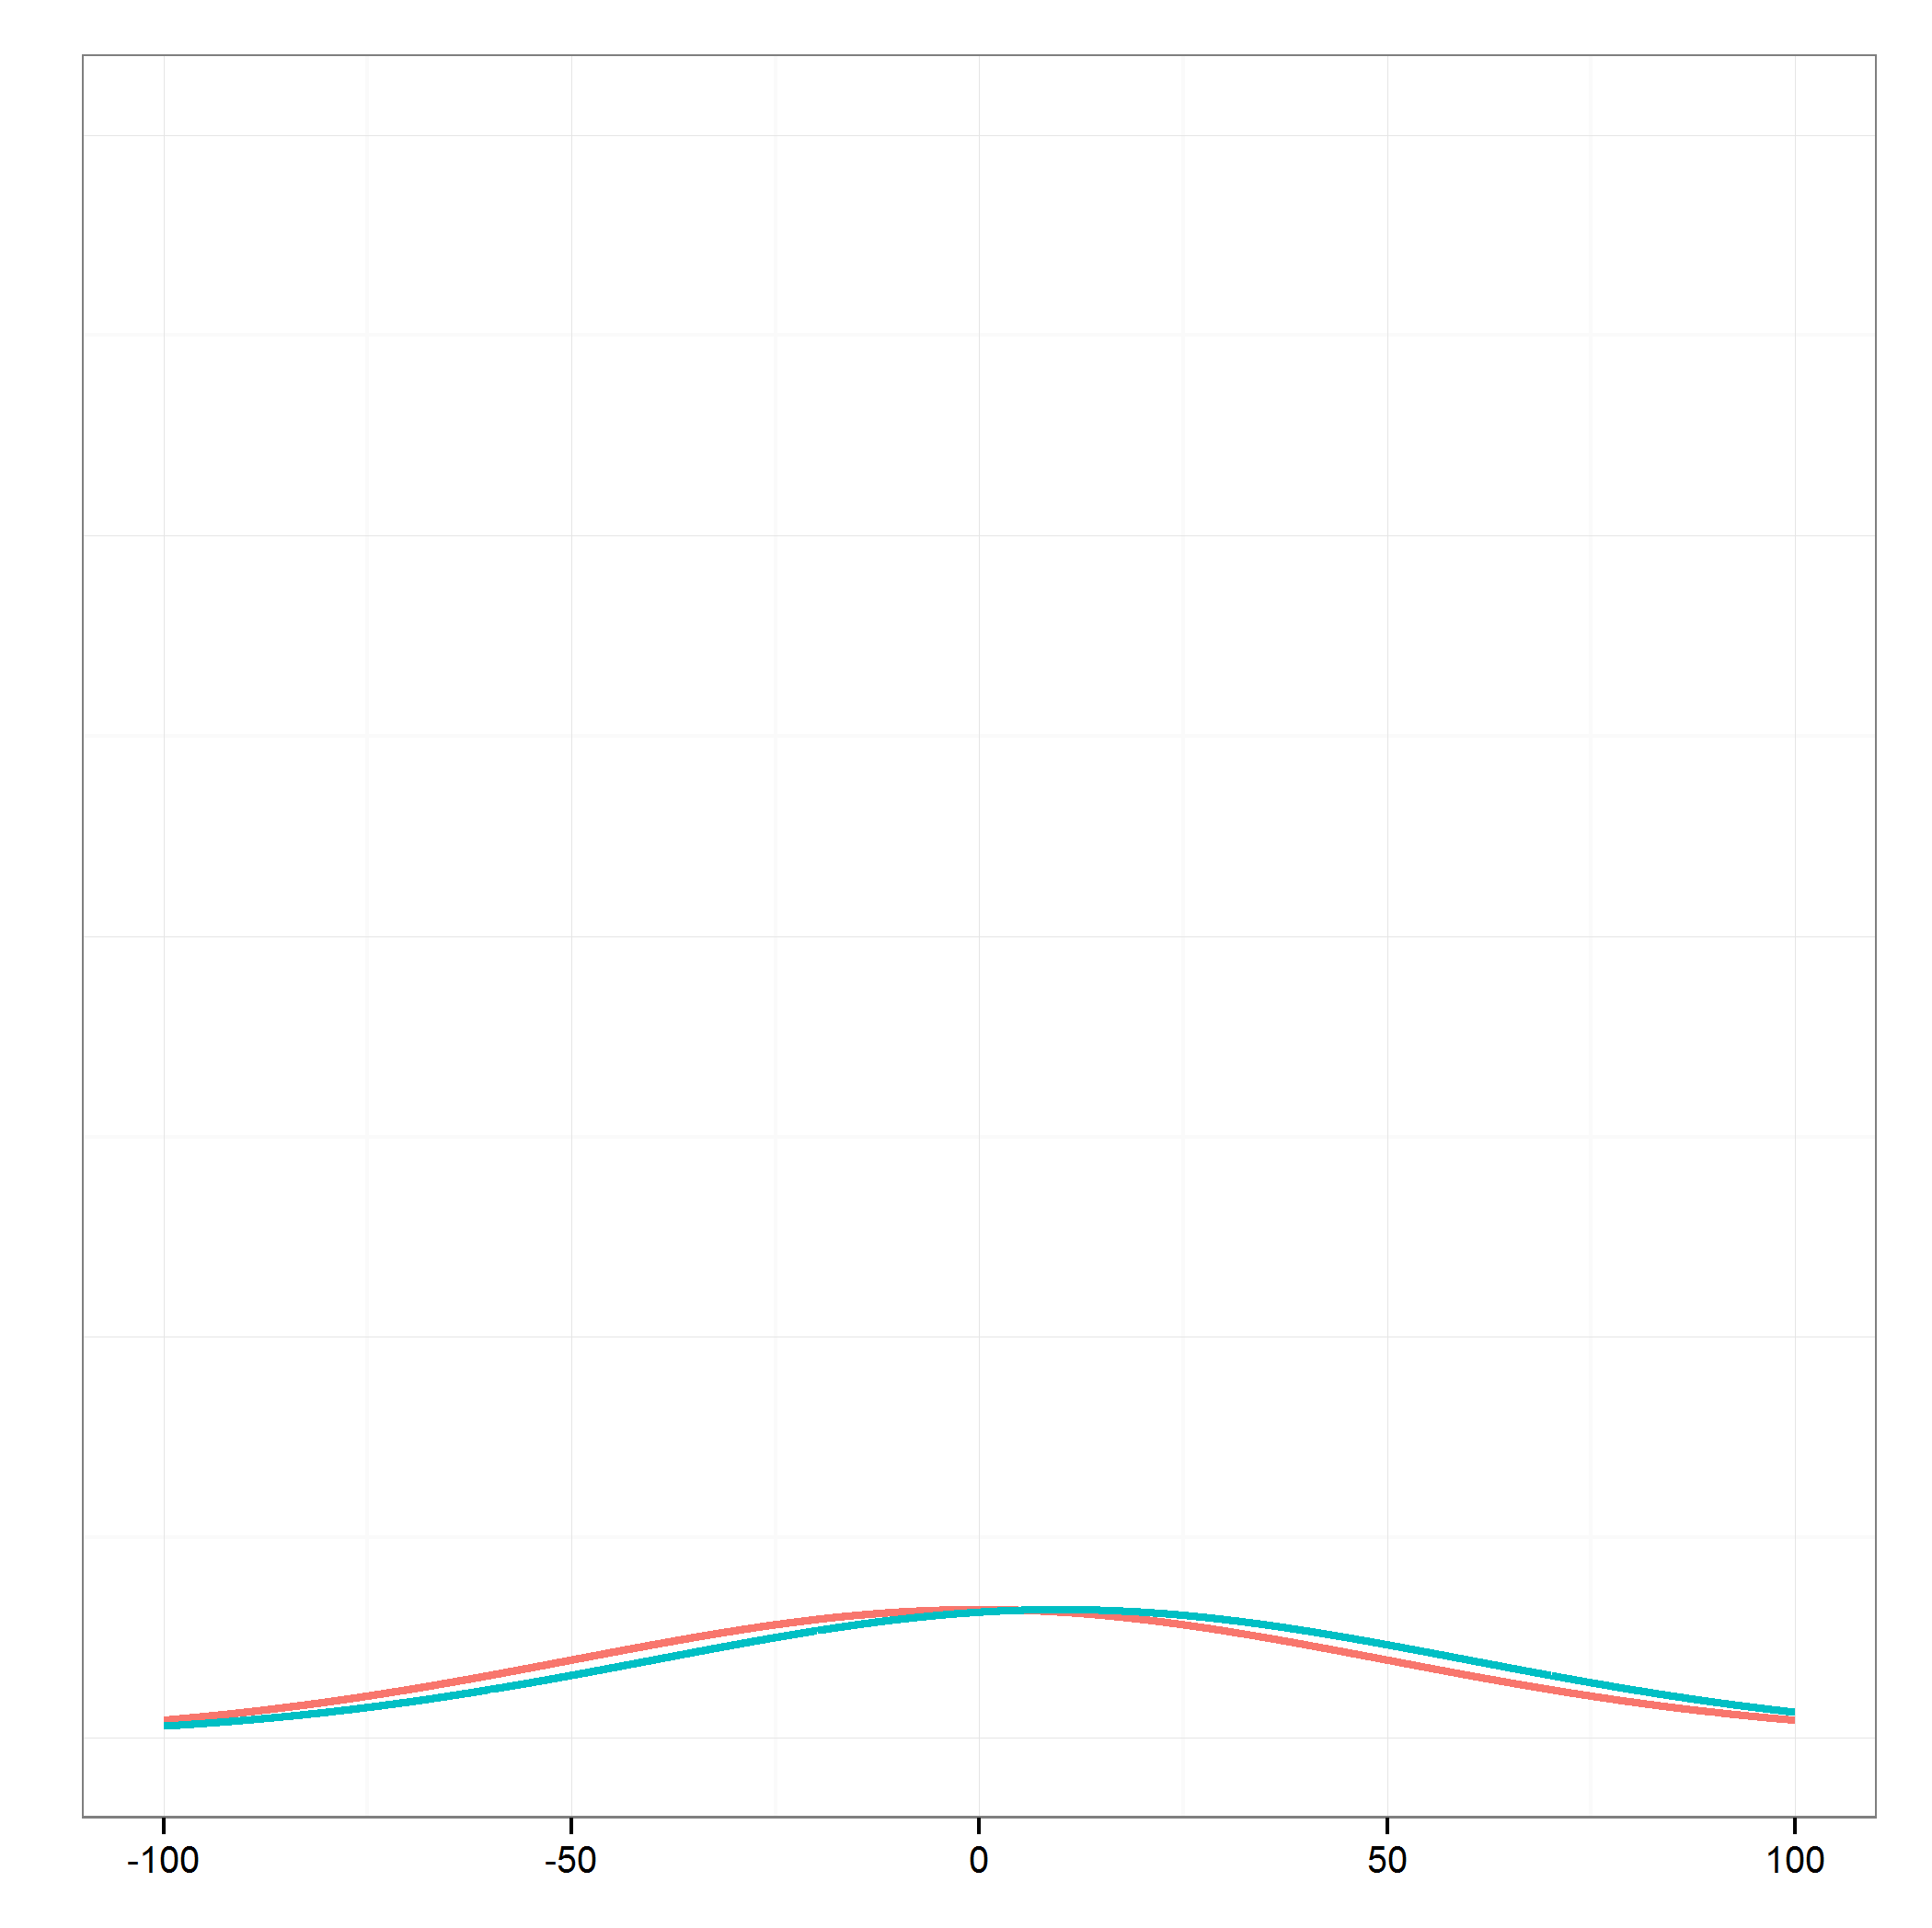
\includegraphics[scale=.3]{figs/first}
\end{block}
\end{column}%
\hfill%
\uncover<2->{
\begin{column}{.48\textwidth}
\begin{block}{\small Low Euclidean distance, High Distribution similarity}
{\small
$\mu_1=0,\sigma_1=0.01$\\
$\mu_2=0.1,\sigma_2=0.01$
}
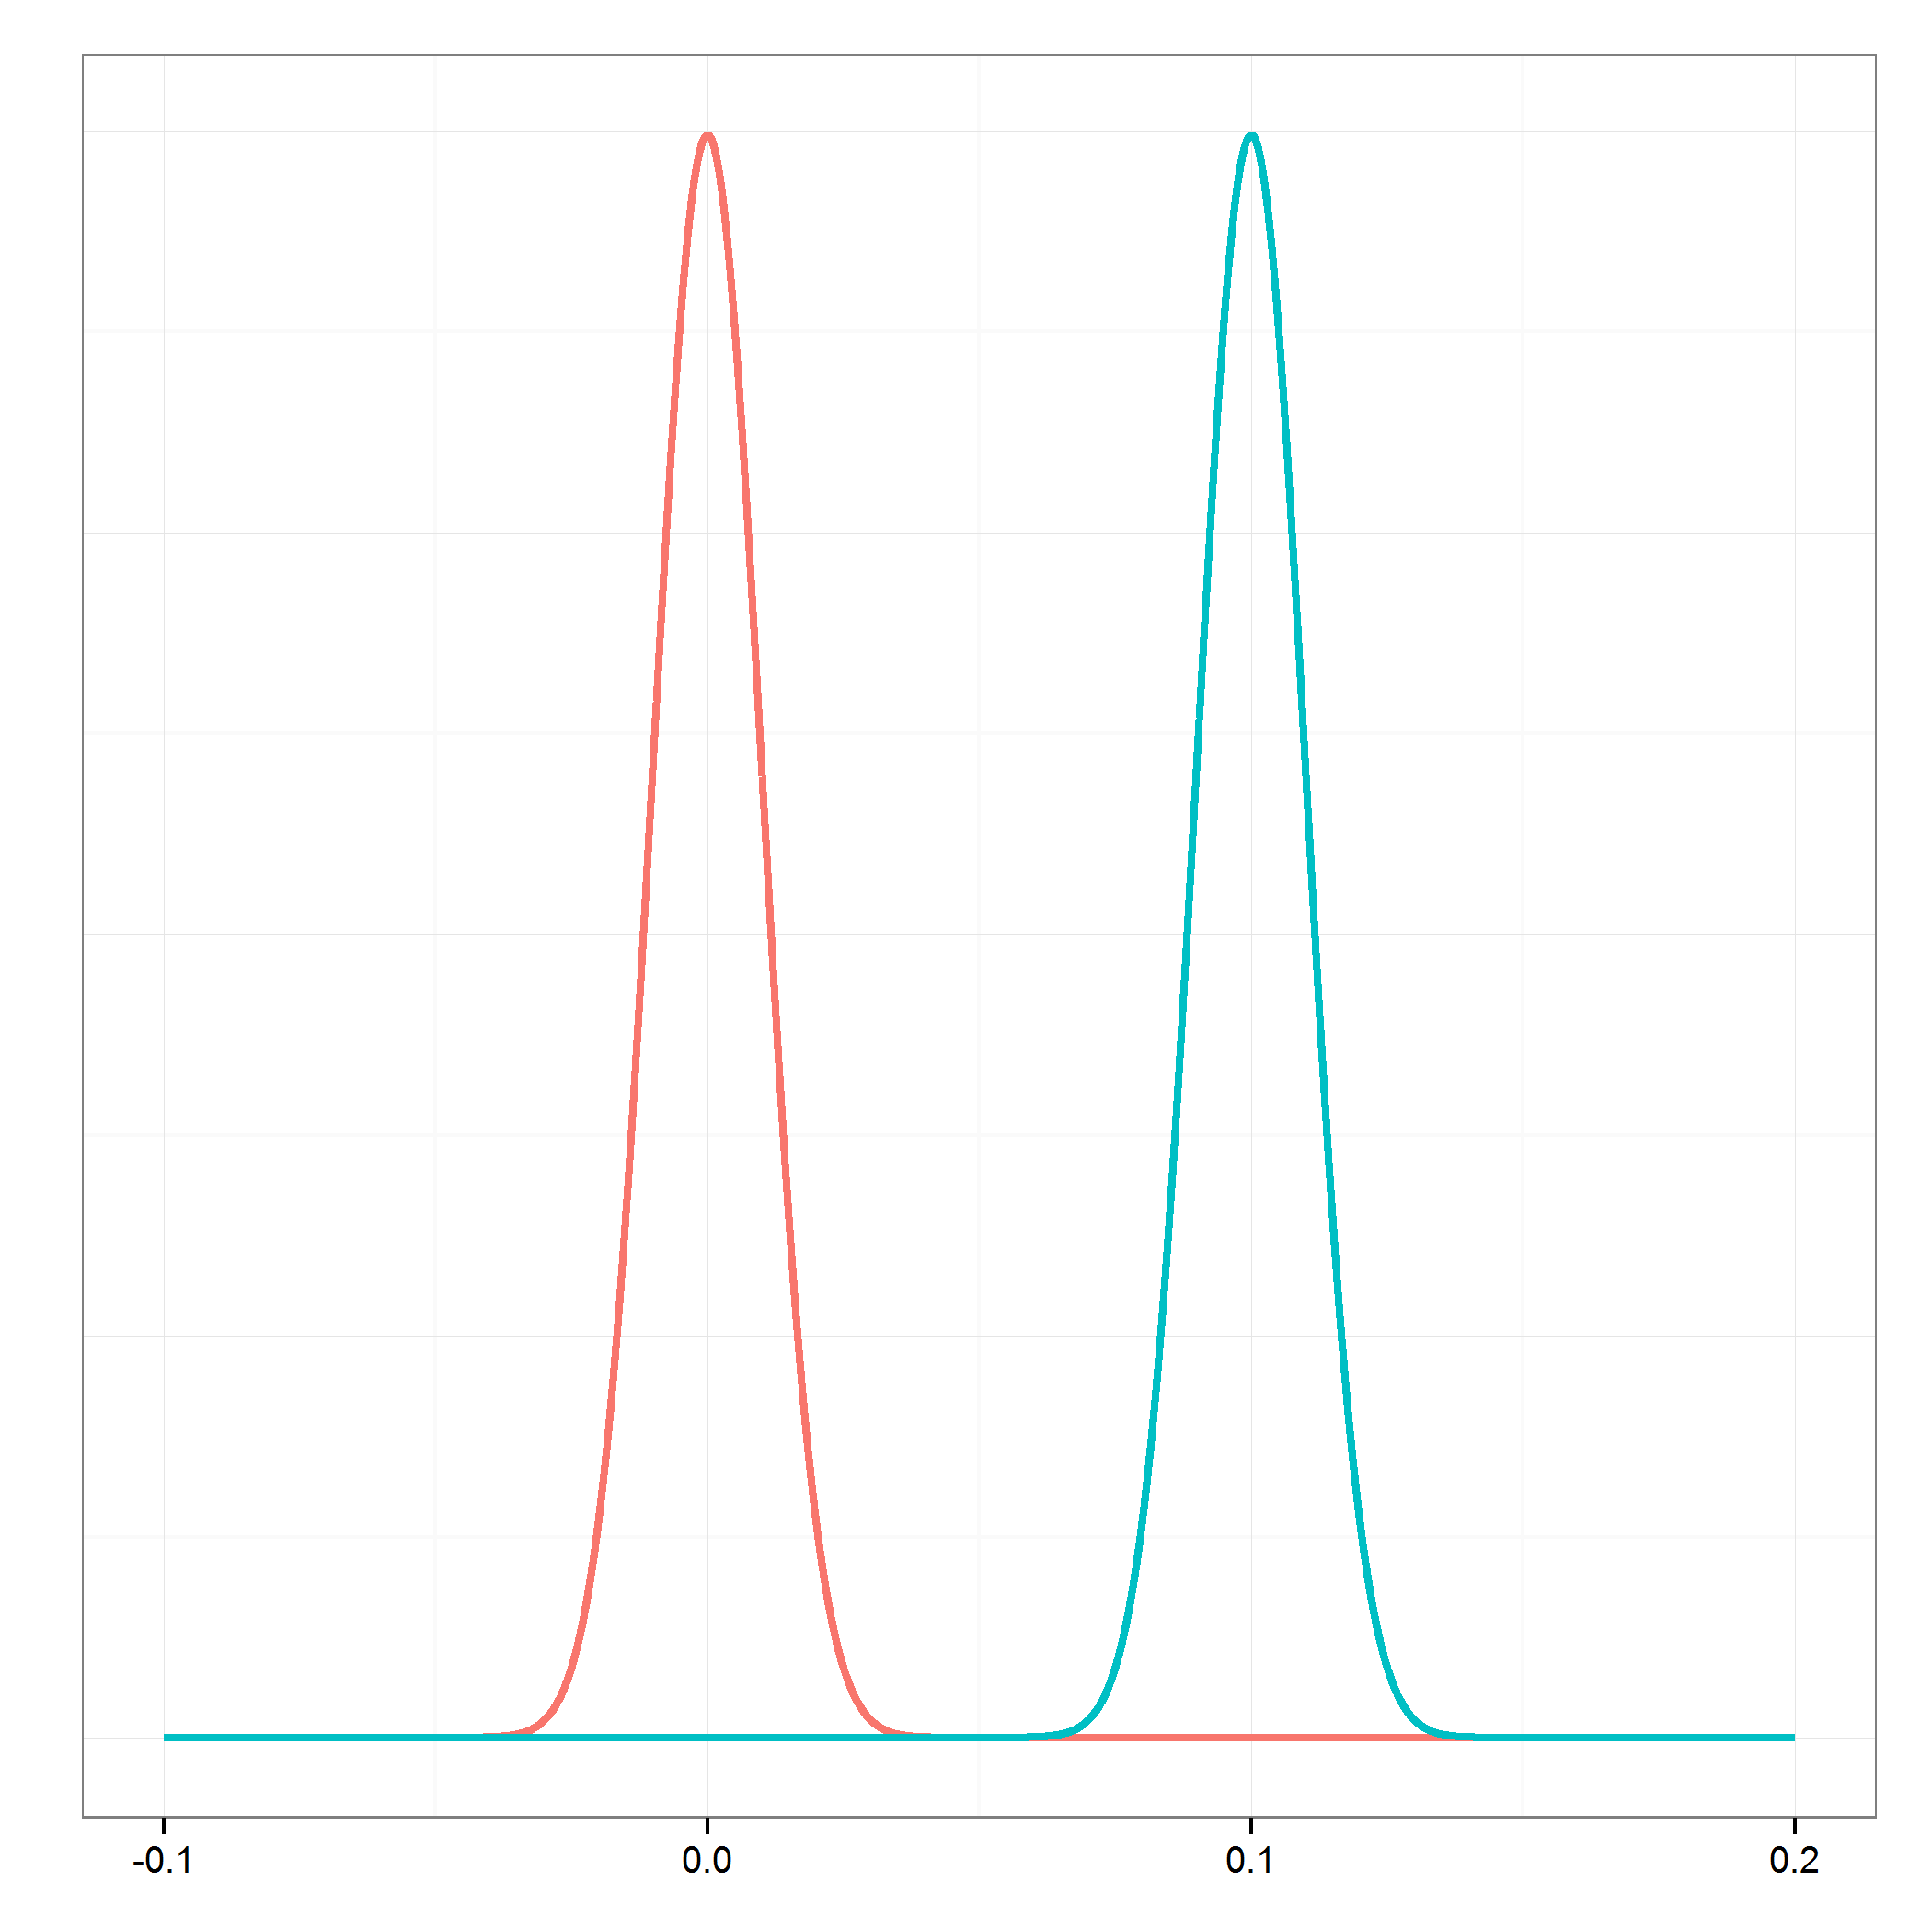
\includegraphics[scale=.3]{figs/second}
\end{block}
\end{column}%
}
\end{columns}
%%%%%%%%%%
}
\frame{\frametitle{Low $D^{\textrm{sym}}_{KL}$ $\approx$ low distribution similarity}
\begin{itemize}
\item  $D^{\textrm{sym}}_{KL}(\lambda_0,\lambda_1) = 
\mathbb{E}_{\lambda_0}\left[ \log{\frac{p_{\lambda_0}}{p_{\lambda_1}} } \right] + 
\mathbb{E}_{\lambda_1}\left[ \log{\frac{p_{\lambda_1}}{p_{\lambda_0}} }\right]$
\item<2-> $p_1 \sim \mathcal{N}(\mu_1,\sigma_1)$, $p_2 \sim \mathcal{N}(\mu_2,\sigma_2)$
\end{itemize}
\uncover<3->{
\begin{columns}
\begin{column}{.48\textwidth}
\begin{block}{\small High Distribution similarity, High $D^{\textrm{sym}}_{KL}$}
{\small
$\mu_1=0,\sigma_1=10K$\\
$\mu_2=10,\sigma_2=10K$\\
$D^{\textrm{sym}}_{KL} = 0.01$\\
}
\begin{center}
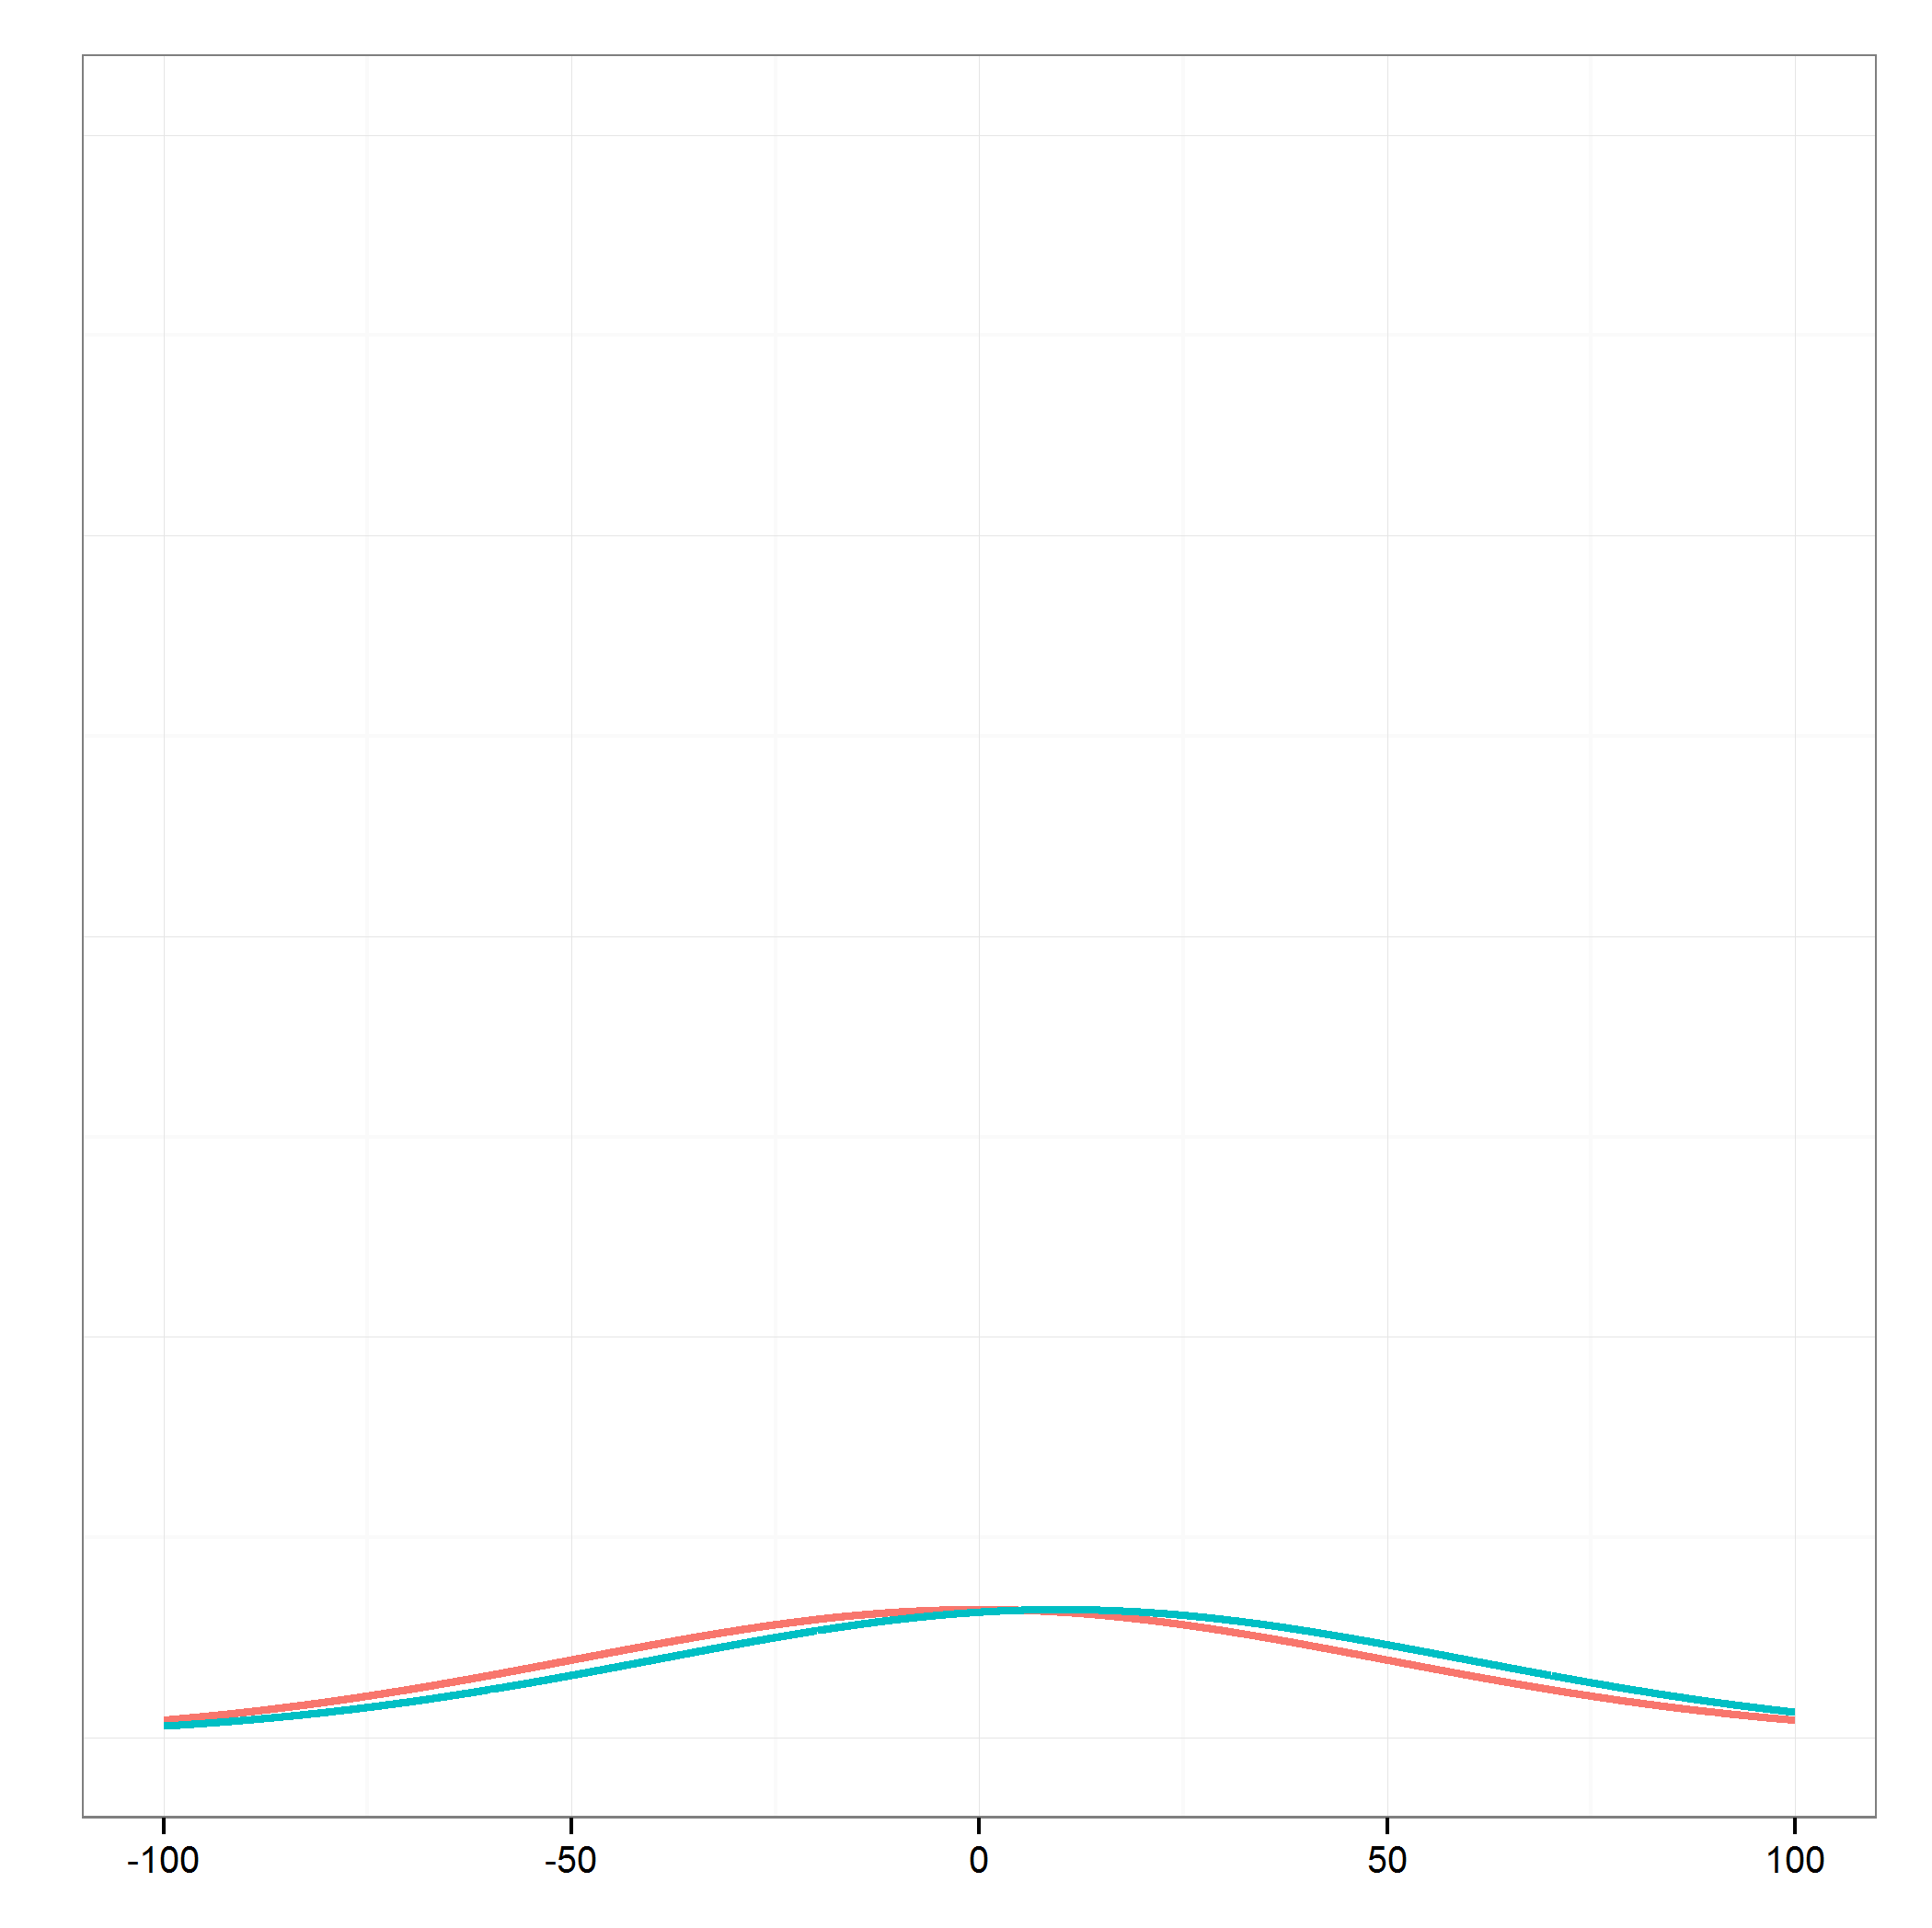
\includegraphics[scale=.15]{figs/first}
\end{center}
\end{block}
\end{column}%
\hfill%
\uncover<4->{
\begin{column}{.48\textwidth}
\begin{block}{\small Low Distribution similarity, Low $D^{\textrm{sym}}_{KL}$}
{\small
$\mu_1=0,\sigma_1=0.01$\\
$\mu_2=0.1,\sigma_2=0.01$\\
$D^{\textrm{sym}}_{KL} = 1$\\
}
\begin{center}
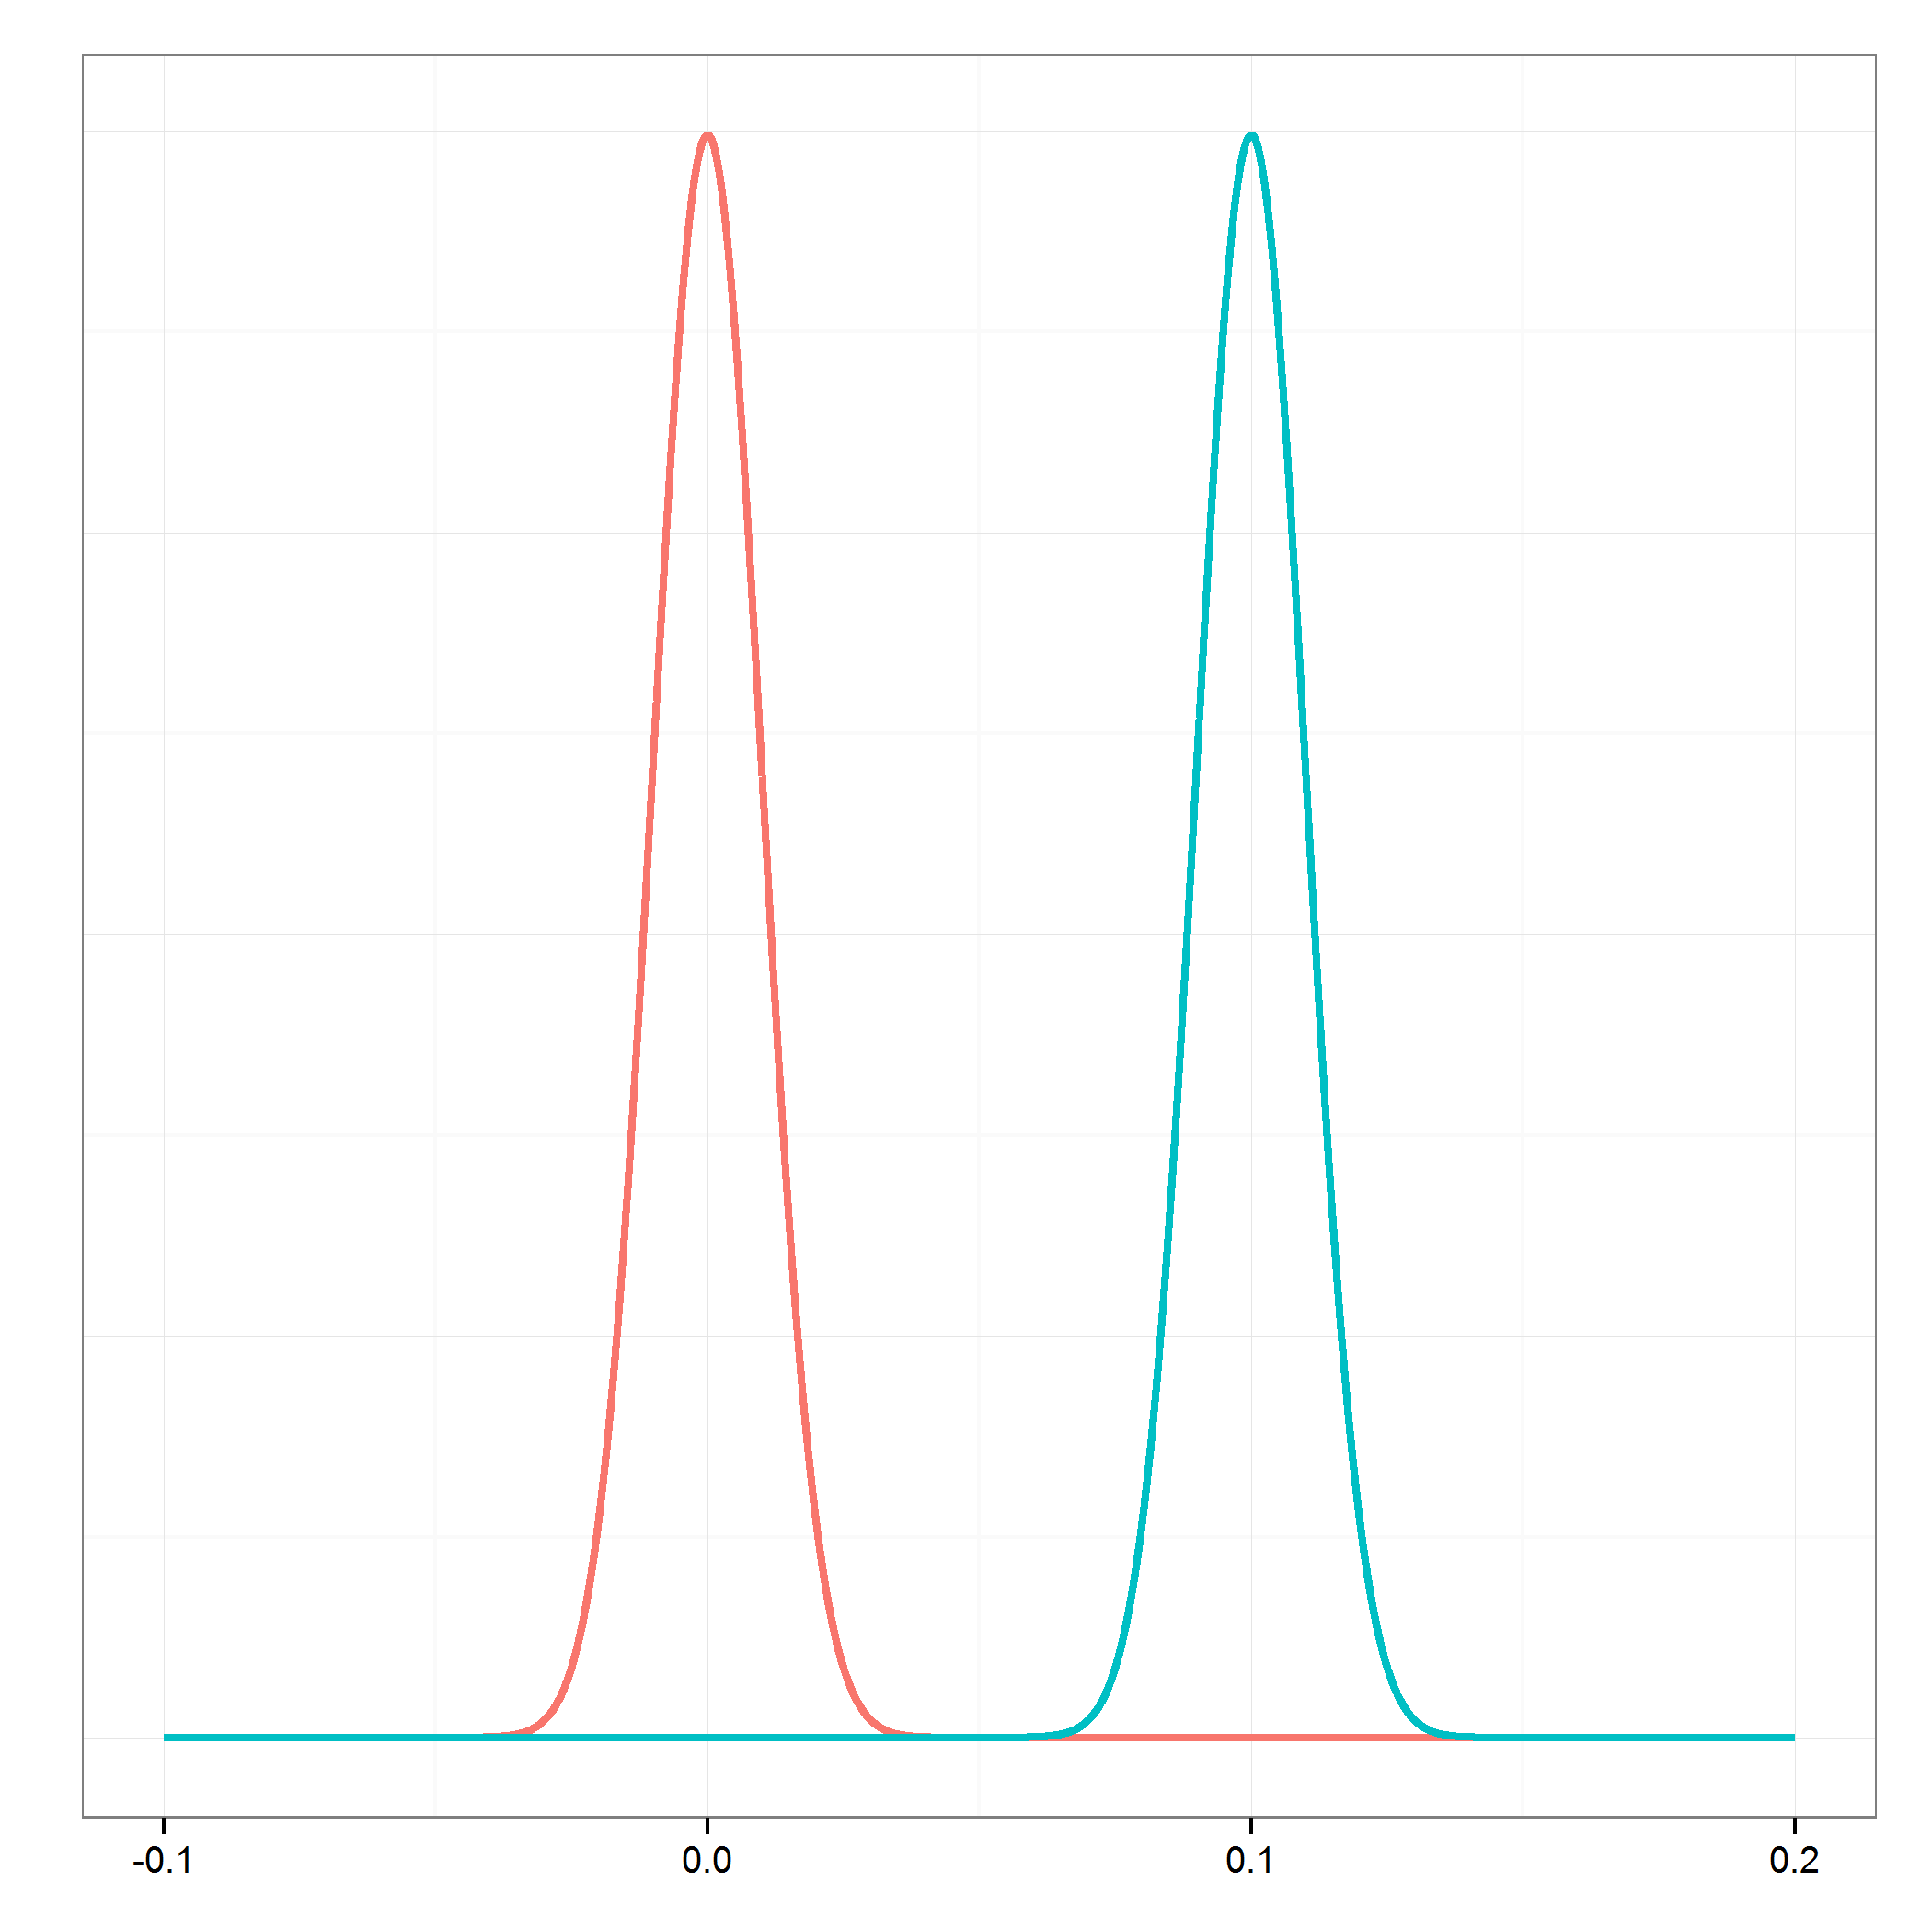
\includegraphics[scale=.15]{figs/second}
\end{center}
\end{block}
\end{column}%
}
\end{columns}
}
%%%%%%%%%%
}
\frame{\frametitle{Natural Gradient}
 Talk about Natural Gradient
}